\documentclass[oneside]{book}

\setcounter{tocdepth}{1}
\setcounter{secnumdepth}{3}

\usepackage[toc,page]{appendix}
\usepackage{hyperref}
\usepackage[utf8]{inputenc}
\usepackage{graphicx} % Required for the inclusion of images
\usepackage{amsmath} % Required for some math elements 
\usepackage[utf8]{inputenc}
\usepackage[english]{babel}
\newtheorem{theorem}{Theorem}
\newtheorem{corollary}{Corollary}[theorem]
\newtheorem{lemma}[theorem]{Lemma}
\usepackage{listings}
\usepackage{pdfpages}
\usepackage{amssymb}
\usepackage{pdflscape}

\begin{document}

\begin{titlepage}
	\centering
	
\includegraphics[width=0.60\textwidth]{../logo/UoN_Primary_Logo_RGB.png}\par\vspace{1cm}
	\vspace{1.5cm}
	{\huge\bfseries Terminology in Functional Agent-Based Simulation \par}
	\vspace{2cm}
	{\Large\itshape jonathan.thaler@nottingham.ac.uk \par}
	\vfill
	
	\vfill

	{\large \today\par}
\end{titlepage}

\cleardoublepage

\chapter{Terminology}

\section*{Abstract}
This document is a collection of the used terminology for the thesis on Functional Agent-Based Simulation. It explains each term, its relevance to the field and the connections to other terms. Included is an A3 poster which visualizes all terms and their connections and can be seen as a mind-map as well.
The intention of this document and poster is to clarify the exact meaning of various terms, their implications and relations to others - to clarify my thinking and discussions.

% TODO: what about an "abstraction" hierarchy? e.g. in this field we have multiple abstraction-layers. e.g. layer 0 paradigms: functional vs. oop, layer 1 languages: haskell vs. java, layer 2 libraries: Yampa (FrABS) vs. Repast Simphony

\clearpage

\section*{Agent}
A pro-active computing-unit with some internal state, which can receive and send messages from other Agents, create new Agents and changes its internal state. It is situated within an Environment with which it can interact directly through reading or writing.

\section*{Environment}
Some generic data which is available to all Agents and can be read and modified by all Agents where the modifications are visible to all Agents. Is not an Agent itself and thus cannot send or receive messages or create new Agents. Although one can see it mostly as being passive, depending on the model, an Environment can also have some behaviour which allows it to e.g. regrow some resources.
The Environment is also the place where to define relations amongst Agents e.g. 2d-discrete/continuous neighbourhood (Moore / Neumann) and/or Networks. Note that an Environment can define and contain multiple relations amongst Agents which can be used by the Agents in different situations.

\section*{Actor}
A weaker form of an Agent which is not able for pro-active behaviour but apart from that identical to an Agent. Was suggested by Carl Hewitt in the 70s as a form of computation. Erlang implements the Actor-Model and Scala comes with an Actor library which supports Actor-based programming.

\section*{Agent-Based Simulation (ABS)}
Simulates a system by simulating its constituting parts, called Agents, and their local interactions. It is assumed that when simulating these local interactions the global dynamics of the system will emerge as an emergent property.
Is used when the global dynamics of a System (Differential Equations) are not known or not feasible to compute \footnote{It is not clear if we can utilize ABS - which is by its very definition of an Agent computable - to simulate a system which dynamics are formalized non-computable.}.
ABS primary advantage over e.g. System Dynamics is that it allows to simulate heterogeneous Agents within an arbitrary and changing environment thus allowing to research spatial- and network-effects and the influence of randomly-distributed properties of the Agents.

\section*{Agent-Based Modelling / Agent-Based Model (ABM)}
Is the process of identifying the constituting parts of a System - the Agents -, their interactions and the Environment in which they are situated in. The result is an Agent-Based Model (ABM) which will reveal its dynamics when computed, resulting in an Agent-Based Simulation (ABS).

\section*{Agent-Based Modelling \& Simulation (ABMS)}
The combination of ABS and ABM.

\section*{Multi-Agent System (MAS)}
Is a software-engineering approach to split a software-system into sub-parts which are implemented as Agents thus resulting in a very decoupled and decentralized software-system. The focus of MAS is often AI (e.g. Belief-Desire-Intention Agents) or Software-Engineering (e.g. Ericsson use of Erlang to implement very high reliable software-systems in telecommunications with up-times of 99.999\%)
A MAS could be used to implement an ABM but MAS are in general very heavy-weight frameworks and bring with it an overhead when just used for simulation. Also they almost always run concurrently, resulting in non-reproducible runs under same starting conditions - something not desirable in ABS.

\section*{Object-Oriented Programming (OO/OOP)}
Is a programming paradigm which builds on the imperative programming paradigm \footnote{There are OO approaches in functional languages e.g. OCAML or F\# but we ignore this here.} organizes the software into objects which send each other messages. The original idea is attributed to Alan Kay where in his original proposal the messages have a share-nothing semantic: no references or mutable state is allowed.
The current popular state-of-the-art OO languages Java and C++ though allow sharing of mutable state and sending of references in messages (=Method-call).
Objects are conceptually quite close to an Agent as they have internal data and provide some interface with which one can interact with them. The main difference is that they are not pro-active and passive: they cannot refuse to process a message sent to them - this power is only available to an Agent or an Actor - and they cannot initiate actions on their own - this is only available to an Agent.
OO also comes with the possibility to define subtype- and object-relations thus can also be understood as a modelling-language.

\section*{Agent-Based Social Simulation (ABSS)}
Simulates social behaviour, societies,...

\section*{Agent-Based Computational Economics (ACE)}
Simulates e.g. trading, economic behaviour amongst Agents.

\section*{Scala}
A multi-paradigm language with focus on functional features, which comes with an Actor-Library and supports Actor-based programming. Can be seen as a more modern version of Erlang.

\section*{Erlang}
A functional language developed by Ericsson to implement high-reliable telecommunication software with up-times of 99.999\%. Implements the Actor-Model.

\section*{Haskell}
A pure functional language with strong static typing. Although primarily used in Academics for programming language, type-system and type-theoretic research, by now it has arrived also in the industry where it demonstrates its usefulness. Also it has heavily influenced other programming languages and introduction of functional features to non-functional languages.

\section*{Functional Programming (FP)}
A programming paradigm based on the lambda calculus which emphasizes a mathematical and declarative approach to programming. In this paradigm one applies arguments to functions and can construct new functions as return-values where these new functions capture values from the returning function.

\section*{Functional Reactive Programming (FRP)}
Allows to program a reactive system in a functional way.

\section*{Yampa}
A library which implements FRP. It supports both discrete and continuous time and is a push-based FRP where the system is sampled with a given time-delta.

\section*{Embedded Domain Specific Language (EDSL)}
In FP when implementing a non-trivial software one strives to implement a so-called EDSL by implementing domain-specific functions which results in a program which looks like a model-specification in that domain. It is called embedded for the reason that this DSL is embedded within a host-language e.g. Haskell (or Scala,...).

\section*{Repast Simphony}
A library for implementing ABS using Java. It provides rich features for importing/exporting data, visualizing dynamics and Agents.

%\begin{landscape}
\centering
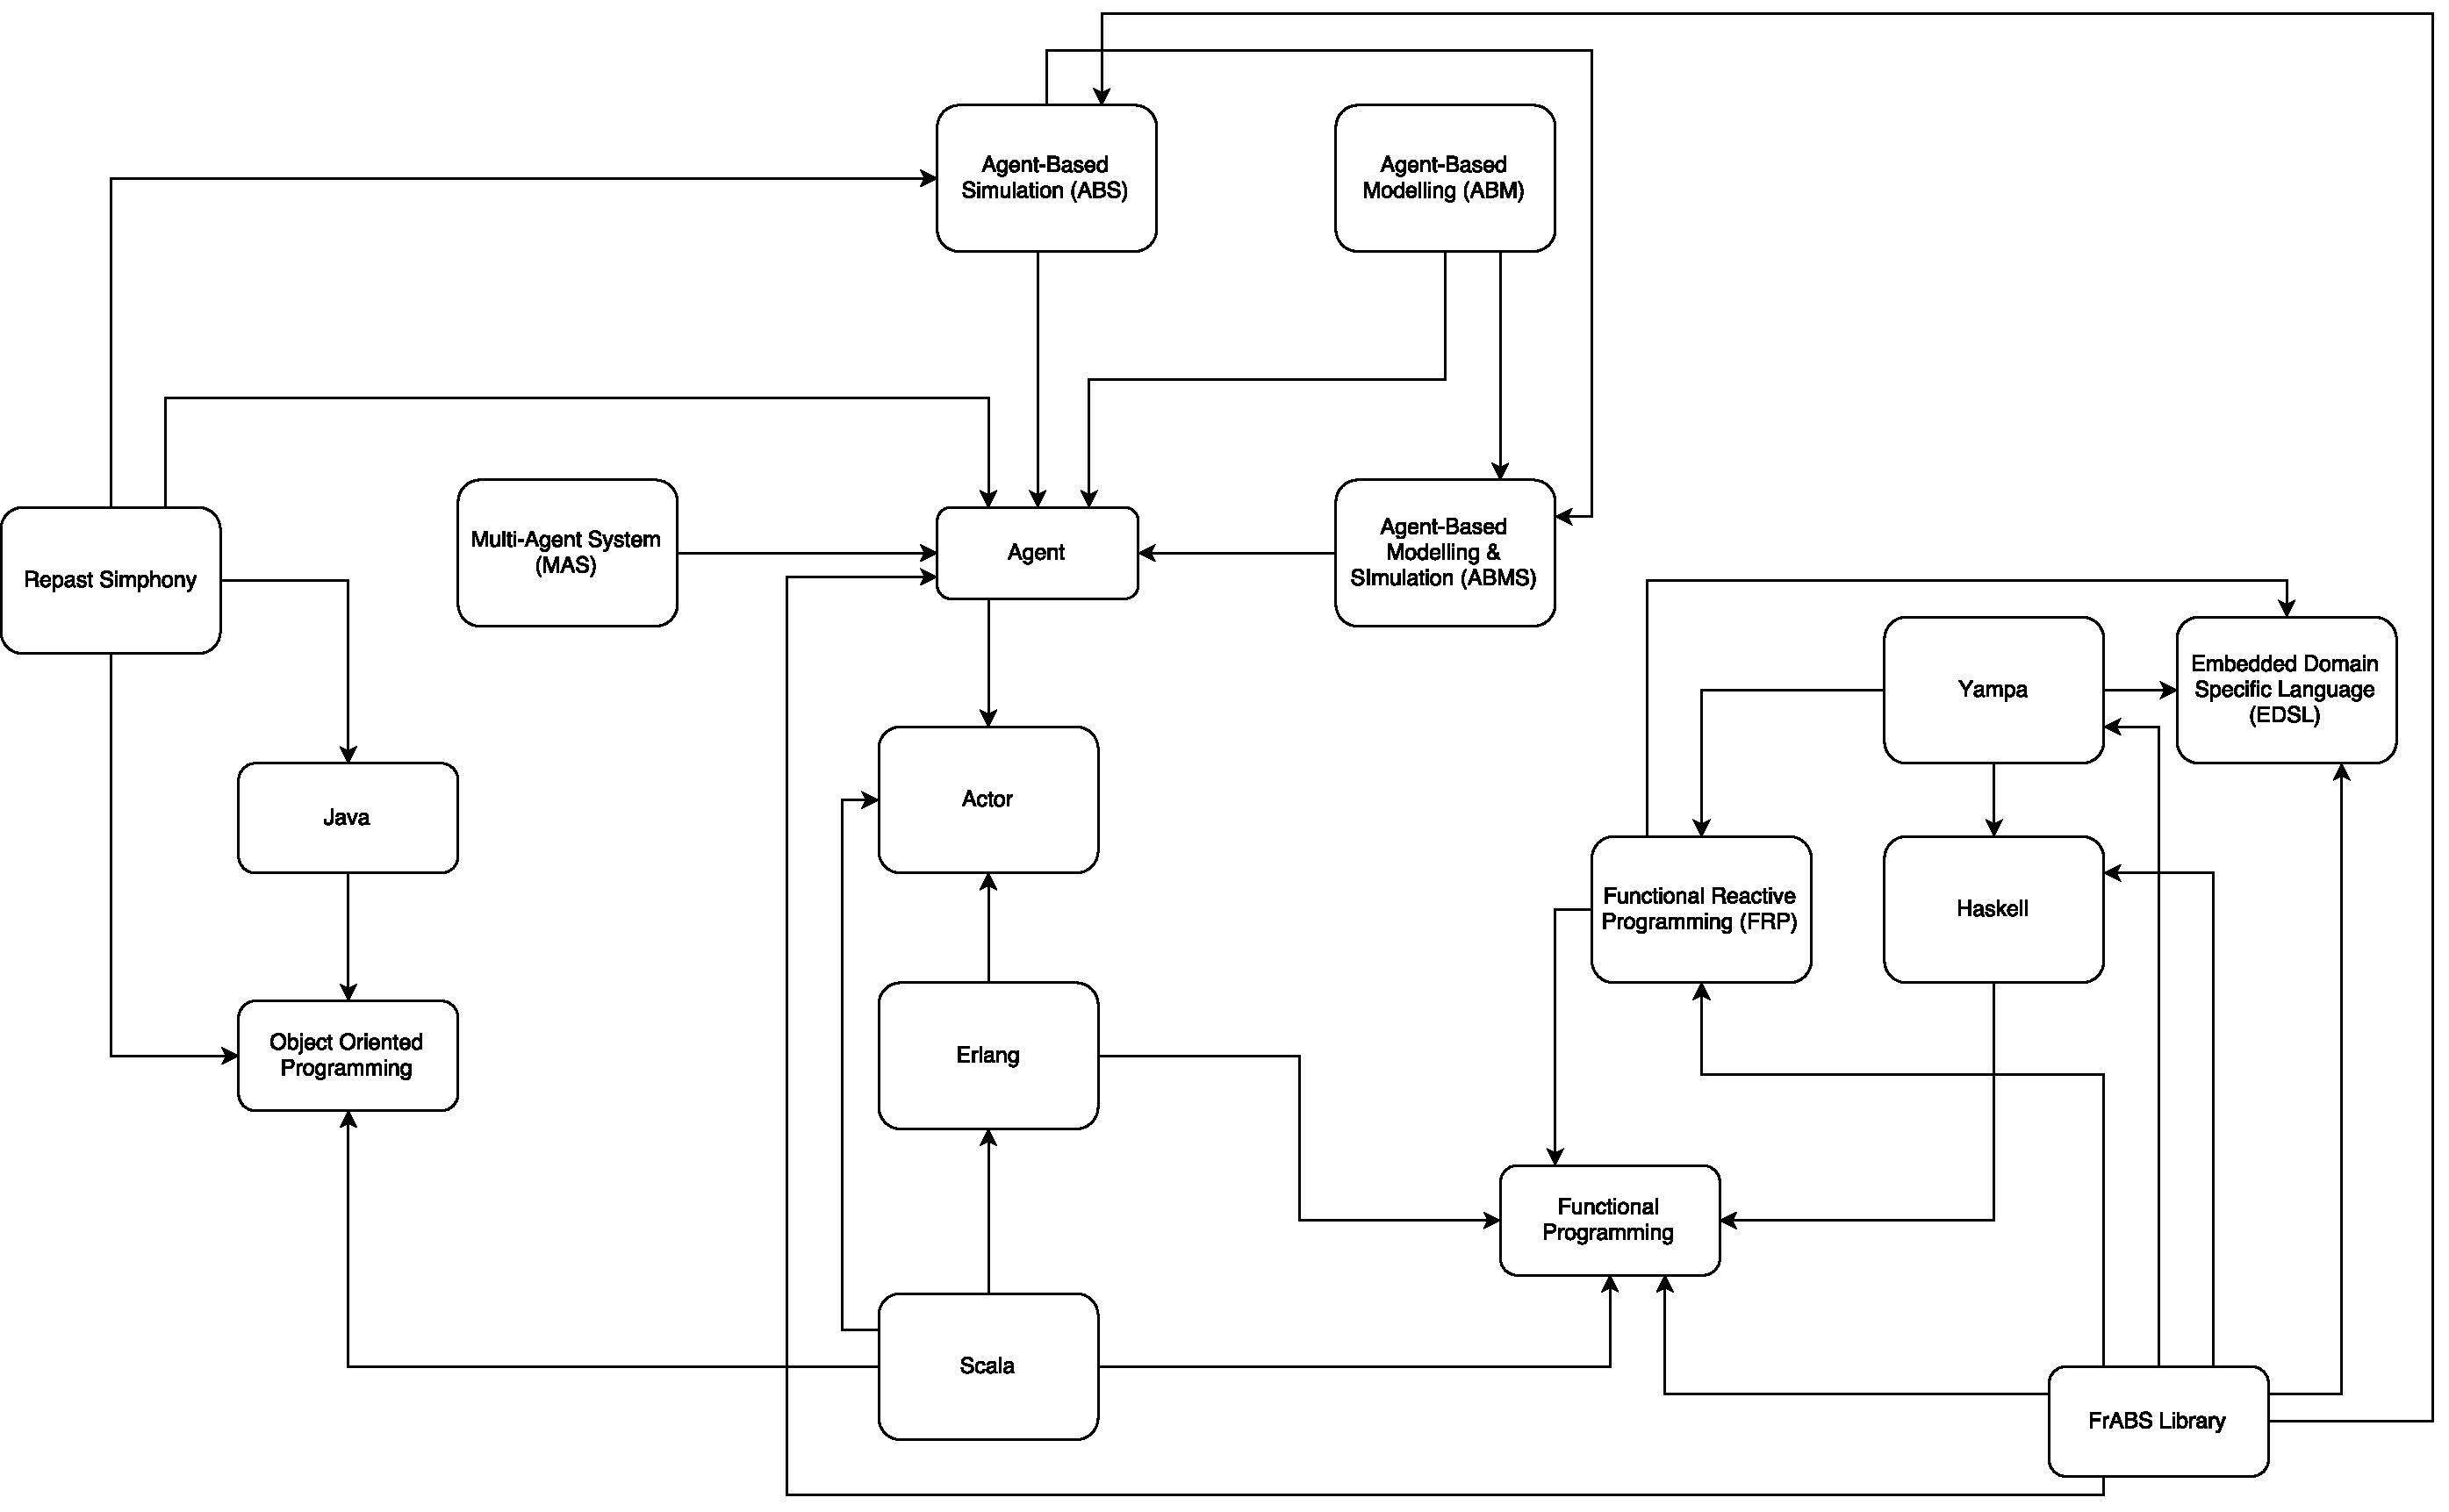
\includepdf[pages=-]{./poster/terminology_relationships.pdf}

%	\begin{figure}
%		\label{fig:gantt}
%  		\caption{Gantt-Chart for remaining PhD}
%  		\centering
%  		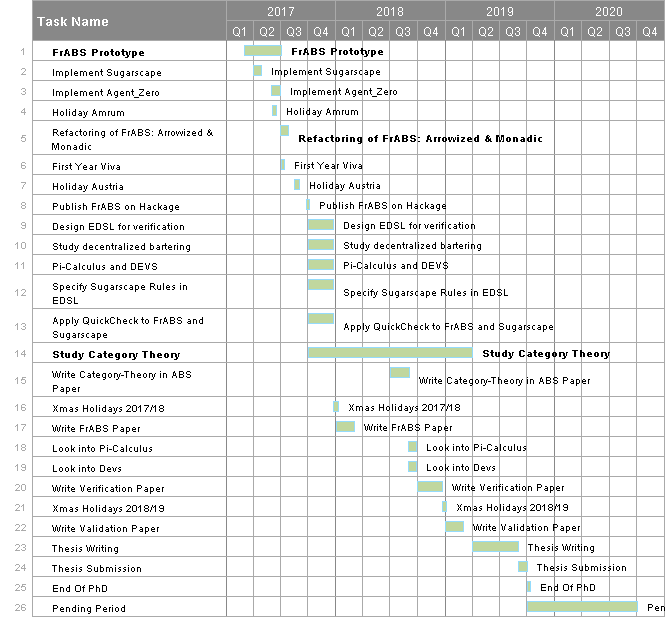
\includegraphics[width=1.2\textwidth]{./charts/gantt.png}
%	\end{figure}
%\end{landscape}

\chapter{Abstraction Layers}
level 0: Lambda Calculus vs. Turing Machine
level 1: FP vs. imperative oop (von neumann, destructive assignment)
level 2: Haskell vs. Java
level 3: FrABS vs. Repast Symphony
level 4: functional ABS vs. oo ABS
level 5: dynamics should be all the same

\end{document}
